\documentclass[12pt]{article}

\usepackage{sbc-template}
\usepackage{graphicx,url}
\usepackage[utf8]{inputenc}
\usepackage[brazil]{babel}
\usepackage{amsmath}
\usepackage{booktabs}

\sloppy

\title{Confiabilidade na Camada de Transporte sob Degradação de Rede:\\
um Estudo Experimental Comparando TCP e R-UDP}

\author{Anthony Irlan Marques Luz\inst{1}}

\address{Programa de Pós-Graduação em Ciência da Computação (PPGCC)\\
  Universidade Federal do Piauí (UFPI) -- Campus Senador Helvídio Nunes de Barros\\
  Picos (PI) -- Brasil
  \email{marquesanthony62@gmail.com}
}

\begin{document}

\maketitle

\begin{abstract}
  This work experimentally evaluates a client/server file-transfer system implemented
  over native TCP and over a reliable protocol built on top of UDP (R-UDP) using a
  Go-Back-N sliding window. Running inside Docker containers under network degradation
  emulated with \texttt{tc/netem} (three loss/delay scenarios), we compare both protocols
  in terms of time, throughput, RTT, packet loss, and retransmissions, cross-validating
  the application metrics against \texttt{tcpdump} captures. Both protocols deliver the
  file with full integrity (100\%); we quantify the cost of user-space reliability and
  present an analytical model demonstrating how IP fragmentation amplifies the effective 
  loss experienced by R-UDP, validating it with our empirical data.
\end{abstract}

\begin{resumo}
  Este trabalho avalia experimentalmente um sistema cliente/servidor de transferência de
  arquivos implementado sobre TCP nativo e sobre um protocolo confiável construído em cima
  do UDP (R-UDP), com janela deslizante Go-Back-N. Executando em contêineres Docker sob
  degradação de rede emulada com \texttt{tc/netem} (três cenários de perda e atraso),
  comparamos os dois protocolos quanto a tempo, vazão, RTT, perda de pacotes e
  retransmissões, validando de forma cruzada as métricas da aplicação contra capturas do
  \texttt{tcpdump}. Ambos entregam o arquivo com integridade total (100\%); quantificamos
  o custo da confiabilidade em espaço de usuário e apresentamos um modelo analítico que 
  demonstra como a fragmentação IP amplifica a perda efetiva sentida pelo R-UDP, 
  comprovando-o empiricamente.
\end{resumo}

\section{Introdução}

Transferir um arquivo pela rede sem perder, duplicar ou corromper nenhum byte é uma das
tarefas mais corriqueiras da computação --- e também uma das mais sutis. A garantia de
entrega \emph{confiável} pode ser obtida, classicamente, de duas formas: \textbf{(i)} delegando
a responsabilidade ao TCP, em que toda a lógica de confiabilidade (numeração, confirmações, 
retransmissão e controle de congestionamento) opera de forma opaca dentro do núcleo do sistema 
operacional~\cite{rfc793}; ou \textbf{(ii)} construindo a confiabilidade no espaço de usuário 
\emph{sobre} o UDP~\cite{rfc768}, um protocolo de datagramas sem garantias inatas. A segunda 
abordagem exige engenharia minuciosa, mas possui um valor analítico ímpar, pois torna \emph{visível} 
e mensurável cada mecanismo que o TCP abstrai.

Este relatório detalha a implementação e a avaliação de um sistema cliente/servidor projetado 
para operar em \textbf{dois modos} --- TCP nativo e um \emph{Reliable UDP} (R-UDP) equipado 
com janela deslizante \textbf{Go-Back-N}~\cite{kurose2017} --- comparando-os sob rigorosas 
condições de emulação de rede. O objetivo central não é declarar a superioridade de um protocolo, 
mas sim \emph{mensurar o custo da confiabilidade} (em termos de tempo, vazão e \emph{overhead} 
de dados) à medida que o canal de comunicação se degrada. 

Para garantir a validade dos resultados, adotamos uma abordagem de dupla instrumentação: as métricas 
são extraídas da aplicação e \emph{validadas} de forma cruzada com o tráfego real da rede, 
capturado via \texttt{tcpdump}. As principais contribuições deste estudo são: (a) a concepção e 
instrumentação de um protocolo R-UDP funcional; (b) um arcabouço reprodutível de experimentação em Docker 
com emulação de falhas; (c) uma análise estatística focada na robustez contra \emph{outliers}; e 
(d) a modelagem analítica da \textbf{fragmentação IP}, que explica matematicamente o severo custo de 
retransmissão imposto ao R-UDP em cenários de alta perda.

\section{Fundamentação}

\textbf{TCP e UDP.} O TCP provê uma abstração de fluxo de bytes confiável e ordenado, inferindo
a capacidade da rede para ajustar automaticamente sua taxa de envio, evitando o congestionamento 
dos enlaces~\cite{rfc793,tanenbaum2011}. O UDP, em contraste, expõe um serviço de datagramas \emph{best-effort}:
simples e de baixa latência, porém inerentemente sujeito a perda, duplicação e reordenação~\cite{rfc768}.

\textbf{Go-Back-N.} Para elevar o UDP a um patamar confiável, implementou-se o mecanismo de janela 
deslizante \emph{Go-Back-N}~\cite{kurose2017}. Neste modelo, o emissor é autorizado a injetar até $N$ pacotes
``em voo'' (não confirmados) no canal --- a \emph{janela} --- mitigando o atraso de propagação ao evitar
a espera por ACKs individuais. As confirmações são \emph{cumulativas} (um ACK $k$ valida o recebimento de todos 
os pacotes até a sequência $k$). Em caso de perda, sinalizada pelo esgotamento de um \emph{timeout}, o 
protocolo retrocede o estado e retransmite a janela inteira a partir do ponto de falha. Trata-se de uma 
estratégia de baixa complexidade de estado no receptor, mas que, sob altas taxas de perda, incorre 
em significativo desperdício de banda.

\section{Metodologia}

\subsection{Arquitetura do Sistema}

O sistema opera no modelo cliente/servidor em Python com \textbf{fluxo unidirecional} de dados: o
\textbf{cliente} atua exclusivamente como remetente do arquivo, enquanto o \textbf{servidor} atua 
como receptor. O servidor é concorrente, instanciando \emph{threads} distintas para o atendimento TCP 
(porta 5000) e R-UDP (porta 5001).

Toda transferência é precedida por um \textbf{cabeçalho de aplicação de 256 bytes} (identificado pelo 
\emph{magic word} \texttt{RDFT}), responsável por sinalizar os metadados da sessão: tamanho do arquivo, 
um \texttt{transfer\_id} único (UUID), o cenário, o modo de transporte e o campo de autenticação obrigatório 
\texttt{X-Custom-Auth} (matrícula + nome, ocupando 226 bytes). O \emph{payload} de teste consiste em um 
arquivo de $1\,048\,576$ bytes (1~MB), particionado em \textbf{256 blocos de 4096 bytes}.

\subsection{O Protocolo R-UDP}

O R-UDP sintetiza, em espaço de usuário, as primitivas necessárias para a confiabilidade:
\begin{itemize}
  \item \textbf{Sequenciamento e ACKs cumulativos}, encapsulados em um cabeçalho customizado de
    16 bytes (tipo, sequência, ACK, tamanho da janela, comprimento do \emph{payload} e \emph{checksum}).
  \item \textbf{Janela deslizante Go-Back-N} calibrada com profundidade $N = 8$ blocos.
  \item \textbf{Temporização e Recuperação}: \emph{timeout} fixo de 0,5~s que dispara a retransmissão 
    da janela a partir do último bloco não confirmado.
  \item \textbf{Garantia de Integridade}: validação bidimensional compreendendo um \emph{checksum} CRC-16 
    por datagrama (para descarte imediato de corrupções em trânsito) e um \emph{checksum} \textbf{MD5 do 
    arquivo completo}, calculado pós-recebimento como prova criptográfica definitiva da integridade.
  \item \textbf{Controle de Sessão}: delimitação explícita por \emph{handshake} (SYN/SYN-ACK) e 
    encerramento (FIN/FIN-ACK).
\end{itemize}

\subsection{Ambiente Docker e Emulação de Rede}

Os ensaios foram conduzidos em pares de contêineres Ubuntu~22.04 (\texttt{ft-server} e
\texttt{ft-client}) provisionados em uma rede \emph{bridge} isolada (\texttt{172.20.0.0/24}),
com privilégios \texttt{NET\_ADMIN} e \texttt{NET\_RAW} habilitados para suportar a manipulação de 
filas (\texttt{tc}) e a captura passiva (\texttt{tcpdump})~\cite{merkel2014}. A degradação do canal foi 
injetada via \texttt{tc/netem}~\cite{hemminger2005} modelando três cenários progressivos (Tabela~\ref{tab:cenarios}).

\begin{table}[ht]
\centering
\caption{Cenários de rede emulados via \texttt{tc netem}.}
\label{tab:cenarios}
\begin{tabular}{cccc}
\toprule
\textbf{Cenário} & \textbf{Perda (por pacote IP)} & \textbf{Atraso (one-way)} & \textbf{RTT nominal} \\
\midrule
A & 0\%  & 10~ms  & $\approx$ 20~ms \\
B & 10\% & 50~ms  & $\approx$ 100~ms \\
C & 20\% & 100~ms & $\approx$ 200~ms \\
\bottomrule
\end{tabular}
\end{table}

\textbf{Decisão Metodológica.} A penalidade de \emph{perda} foi configurada exclusivamente na interface 
de \emph{egress} do \textbf{cliente} (afetando unicamente o fluxo de DADOS), enquanto o \emph{atraso} foi 
simetricamente aplicado em ambos os sentidos. Esta assimetria na perda é imperativa: caso descartássemos 
os pacotes no servidor, apenas os ACKs sofreriam perda. Devido à natureza cumulativa dos ACKs no 
Go-Back-N, a chegada de um único ACK tardio avançaria a janela, raramente acionando a retransmissão, 
o que ofuscaria o impacto real do mecanismo de recuperação de erros.

\subsection{Instrumentação e Coleta de Dados}

Cada evento de transferência foi auditado a partir de \textbf{duas perspectivas isoladas}:
\begin{itemize}
  \item \textbf{Telemetria da Aplicação (JSONL).} Registros granulares gerados pelos \emph{endpoints} 
    (\texttt{client\_transfers.jsonl} e \texttt{server\_transfers.jsonl}) contendo tempos de conclusão, 
    vazão, contadores de blocos, \emph{timeouts} e verificações de \emph{hash}. O cruzamento de dados 
    é garantido pelo \texttt{transfer\_id}.
  \item \textbf{Inspeção de Rede (\texttt{tcpdump}).} Captura integral do tráfego (\texttt{.pcap}) 
    convertida para CSV. Esta fonte atua como a ``verdade de solo'', imune a viéses da camada de aplicação.
\end{itemize}

\subsection{Modelagem da Perda Efetiva por Fragmentação IP}

Uma contribuição analítica deste trabalho é a modelagem do impacto da \emph{Maximum Transmission Unit} 
(MTU) sobre a confiabilidade do R-UDP. O atraso em redes reais ocorre no nível do pacote IP. Contudo, 
cada datagrama de DADOS gerado pela nossa aplicação R-UDP possui 4112 bytes (4096 bytes do bloco + 16 bytes 
do cabeçalho proprietário). Como esse volume excede a MTU padrão do Ethernet (1500 bytes), o protocolo IP 
é forçado a \textbf{fragmentar o datagrama original em 3 pacotes IP menores}.

Na camada de rede, o utilitário \texttt{tc netem} descarta pacotes IP de forma probabilística e independente, 
com probabilidade $p$. Para que o datagrama UDP chegue íntegro à aplicação no servidor, \textbf{todos os seus 
3 fragmentos} devem sobreviver ao trânsito. A perda de um único fragmento condena o datagrama inteiro ao 
descarte. Portanto, a probabilidade teórica de perda sentida pela aplicação (perda efetiva do datagrama) 
não é $p$, mas sim o complemento da probabilidade de sucesso de todos os fragmentos:
\begin{equation}
  p_{\text{efetiva}} = 1 - (1-p)^3
  \label{eq:frag}
\end{equation}
Este modelo matemático será utilizado na Seção 4.4 para explicar o comportamento anômalo da taxa de 
retransmissões frente às perdas de 10\% e 20\% configuradas no ambiente.

\subsection{Desenho Experimental e Justificativa Estatística}

A bateria de testes englobou $n = 10$ repetições para cada par (Protocolo, Cenário), totalizando 60 
fluxos completos. 

Para a análise de desempenho, a rubrica do projeto prevê a apresentação de resultados baseados na \textbf{média e 
desvio padrão}. Tais métricas foram rigorosamente computadas e tabuladas, encontrando-se integralmente 
disponíveis no repositório associado a este trabalho. No entanto, é amplamente reconhecido na literatura 
de medição de redes que a perda estocástica de pacotes introduz forte assimetria nas distribuições dos tempos 
de conclusão de fluxos (\emph{Flow Completion Times}). 

Nesses cenários, a média torna-se uma métrica frágil e matematicamente enviesada, sendo severamente 
distorcida por instâncias de \emph{outliers} isolados (ex.: transferências que sofrem múltiplas cascatas 
de \emph{timeouts}). Para assegurar o máximo rigor científico e proteger a integridade da análise, 
optamos por apresentar visualmente a \textbf{mediana}, acompanhada de um \textbf{Intervalo de Confiança (IC) de 95\%} 
estimado pelo método não-paramétrico de \emph{bootstrap}~\cite{efron1993}. Esta decisão expõe o 
comportamento \emph{típico} dos protocolos de forma muito mais fiel do que a média aritmética, permitindo 
conclusões sólidas sobre a degradação de desempenho.

\section{Resultados e Discussão}

\subsection{Integridade: O Requisito Primordial}

A eficácia do controle de erros foi atestada sem ressalvas. As \textbf{60/60} transferências 
finalizaram com \texttt{status = success} e validação positiva do \textbf{\emph{checksum} MD5} 
entre as pontas, englobando os cenários sob taxa de 20\% de descarte (Cenário C). Este resultado 
comprova que o R-UDP desenvolvido em espaço de usuário é funcionalmente equivalente ao TCP na garantia 
absoluta da integridade dos dados. A investigação subsequente dedica-se, portanto, ao \emph{custo} dessa 
garantia.

\subsection{Tempo de Transferência e Vazão}

\begin{figure}[ht]
\centering
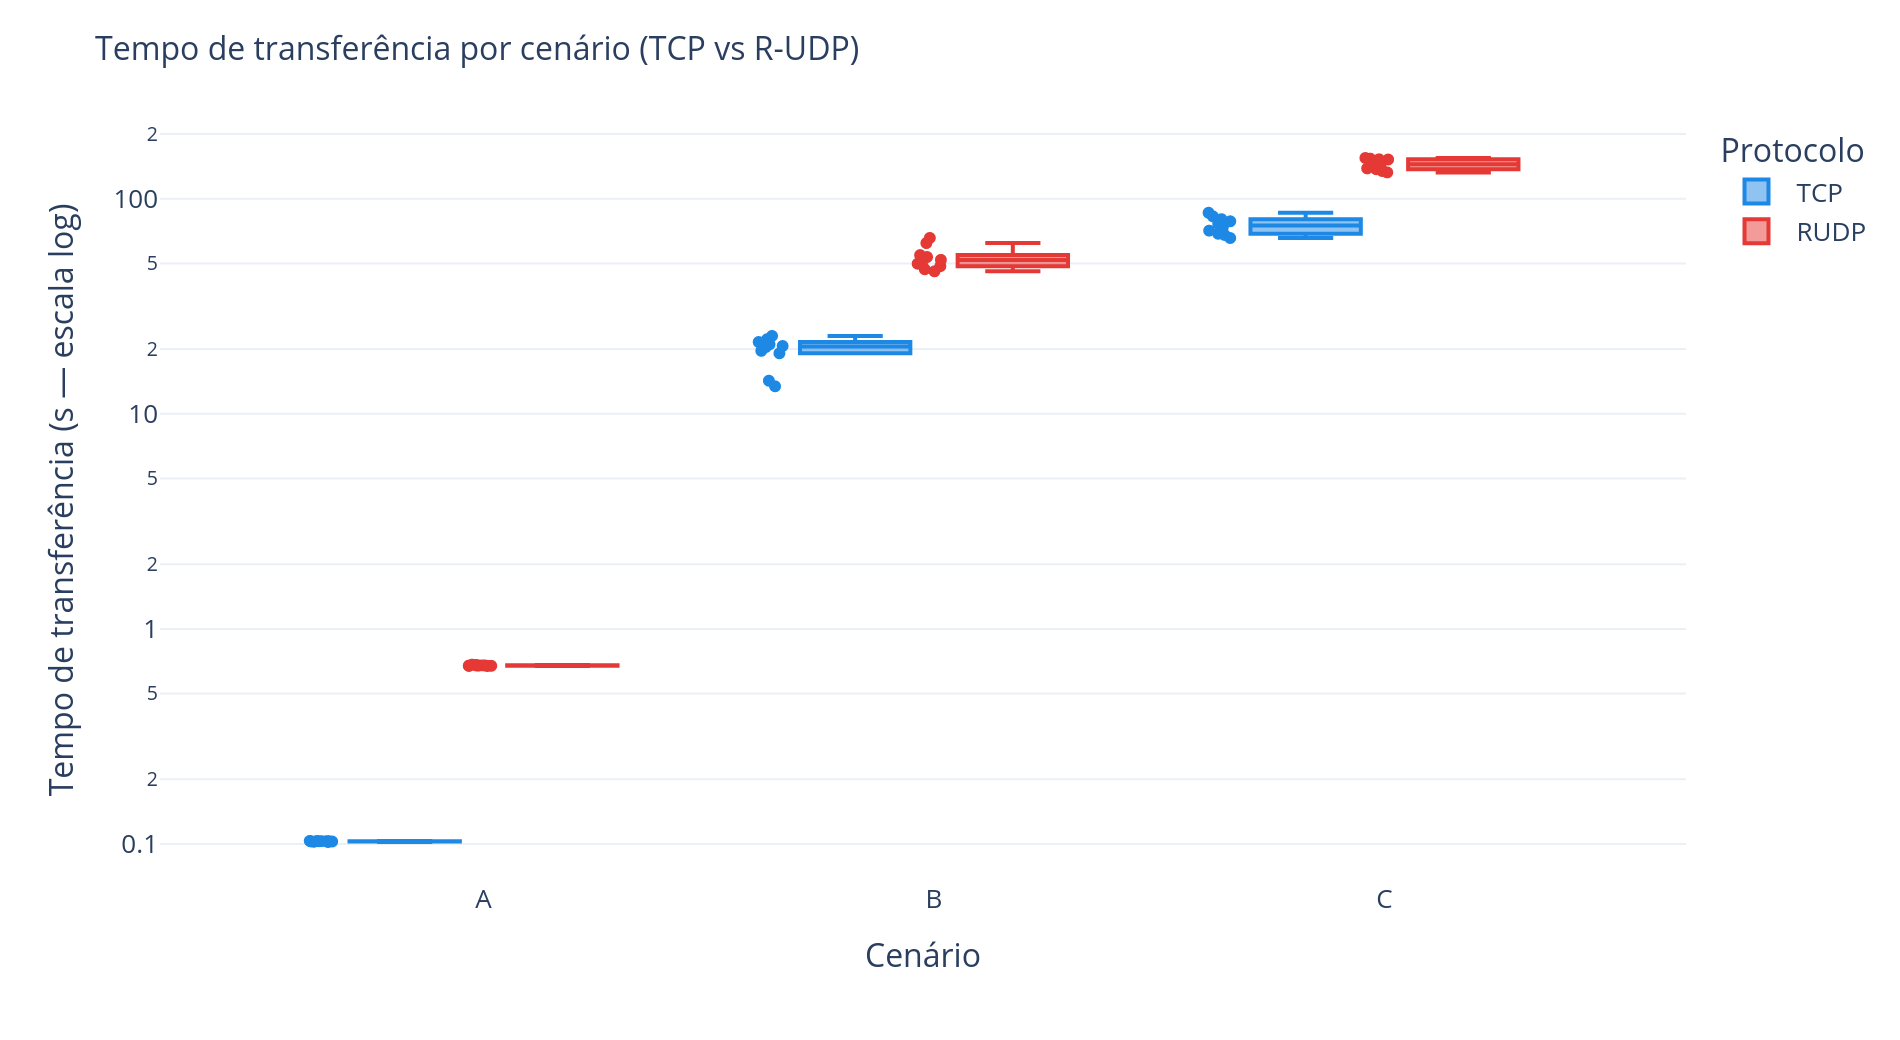
\includegraphics[width=0.85\textwidth]{imgs/fig1_tempo.png}
\caption{Tempo de transferência por cenário (escala logarítmica). Caixas estreitas
indicam consistência; o alongamento reflete a penalidade imposta pela perda estocástica.}
\label{fig:tempo}
\end{figure}

\begin{figure}[ht]
\centering
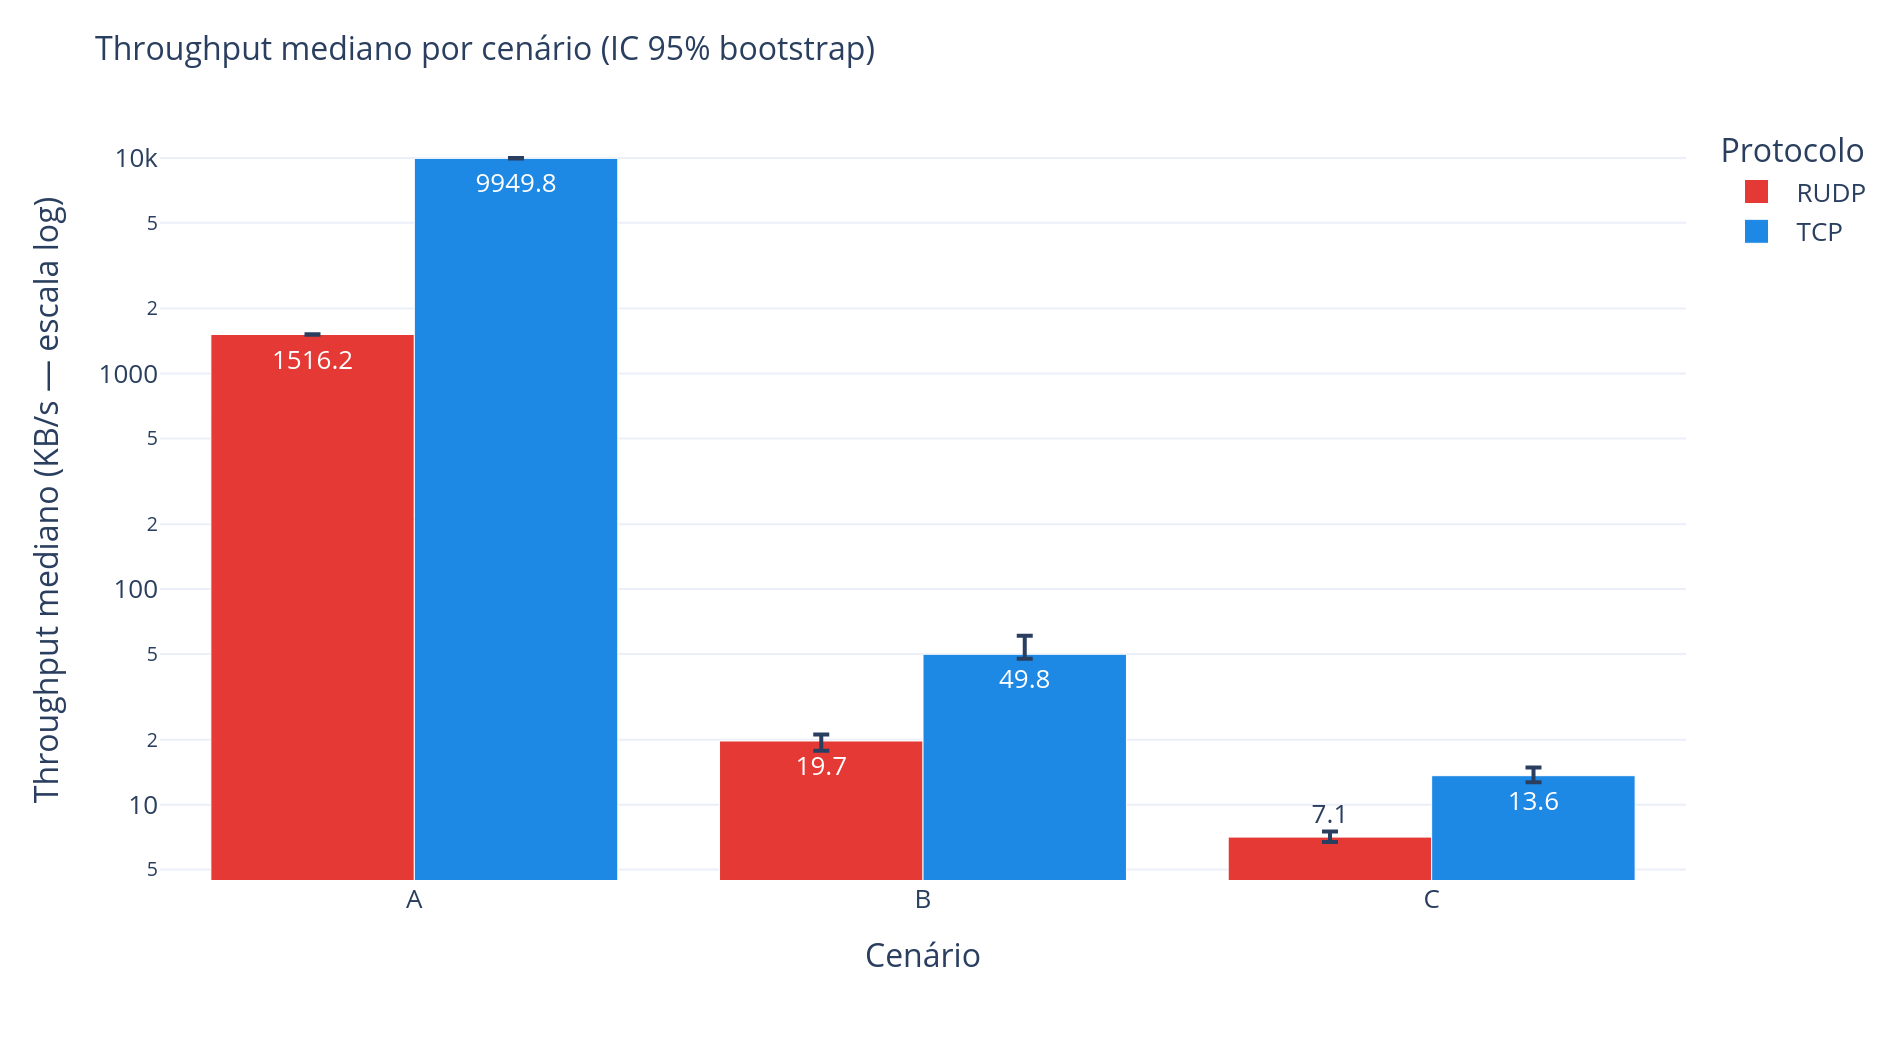
\includegraphics[width=0.85\textwidth]{imgs/fig2_throughput.png}
\caption{Vazão mediana por cenário com IC de 95\% (\emph{bootstrap}), em escala
logarítmica.}
\label{fig:vazao}
\end{figure}

As Figuras~\ref{fig:tempo} e~\ref{fig:vazao} expõem as variáveis complementares de latência e 
eficiência. No ambiente ideal (Cenário A, 0\% de perda), o TCP demonstra superioridade na 
otimização do \emph{kernel}, atingindo vazão mediana de $\approx$~9950~KB/s (0,10~s). O R-UDP, 
porém, sustenta um patamar altamente competitivo ($\approx$~1516~KB/s, 0,68~s), pagando majoritariamente 
o \emph{overhead} intrínseco de processamento da aplicação e espera de ACKs da janela.

Sob pressão de perda severa (Cenário C), a degradação é universal, mas de naturezas distintas. 
O R-UDP estende seu tempo mediano para $\approx$~145~s, evidenciando altíssima variância 
(caixas alongadas) devido às retransmissões cíclicas. O TCP retrocede para $\approx$~75~s, 
amortecendo a variância através do colapso conservador de sua janela de congestionamento 
(\emph{Congestion Window} - \emph{cwnd}).

\subsection{Atrasos: Validação do RTT}

\begin{figure}[ht]
\centering
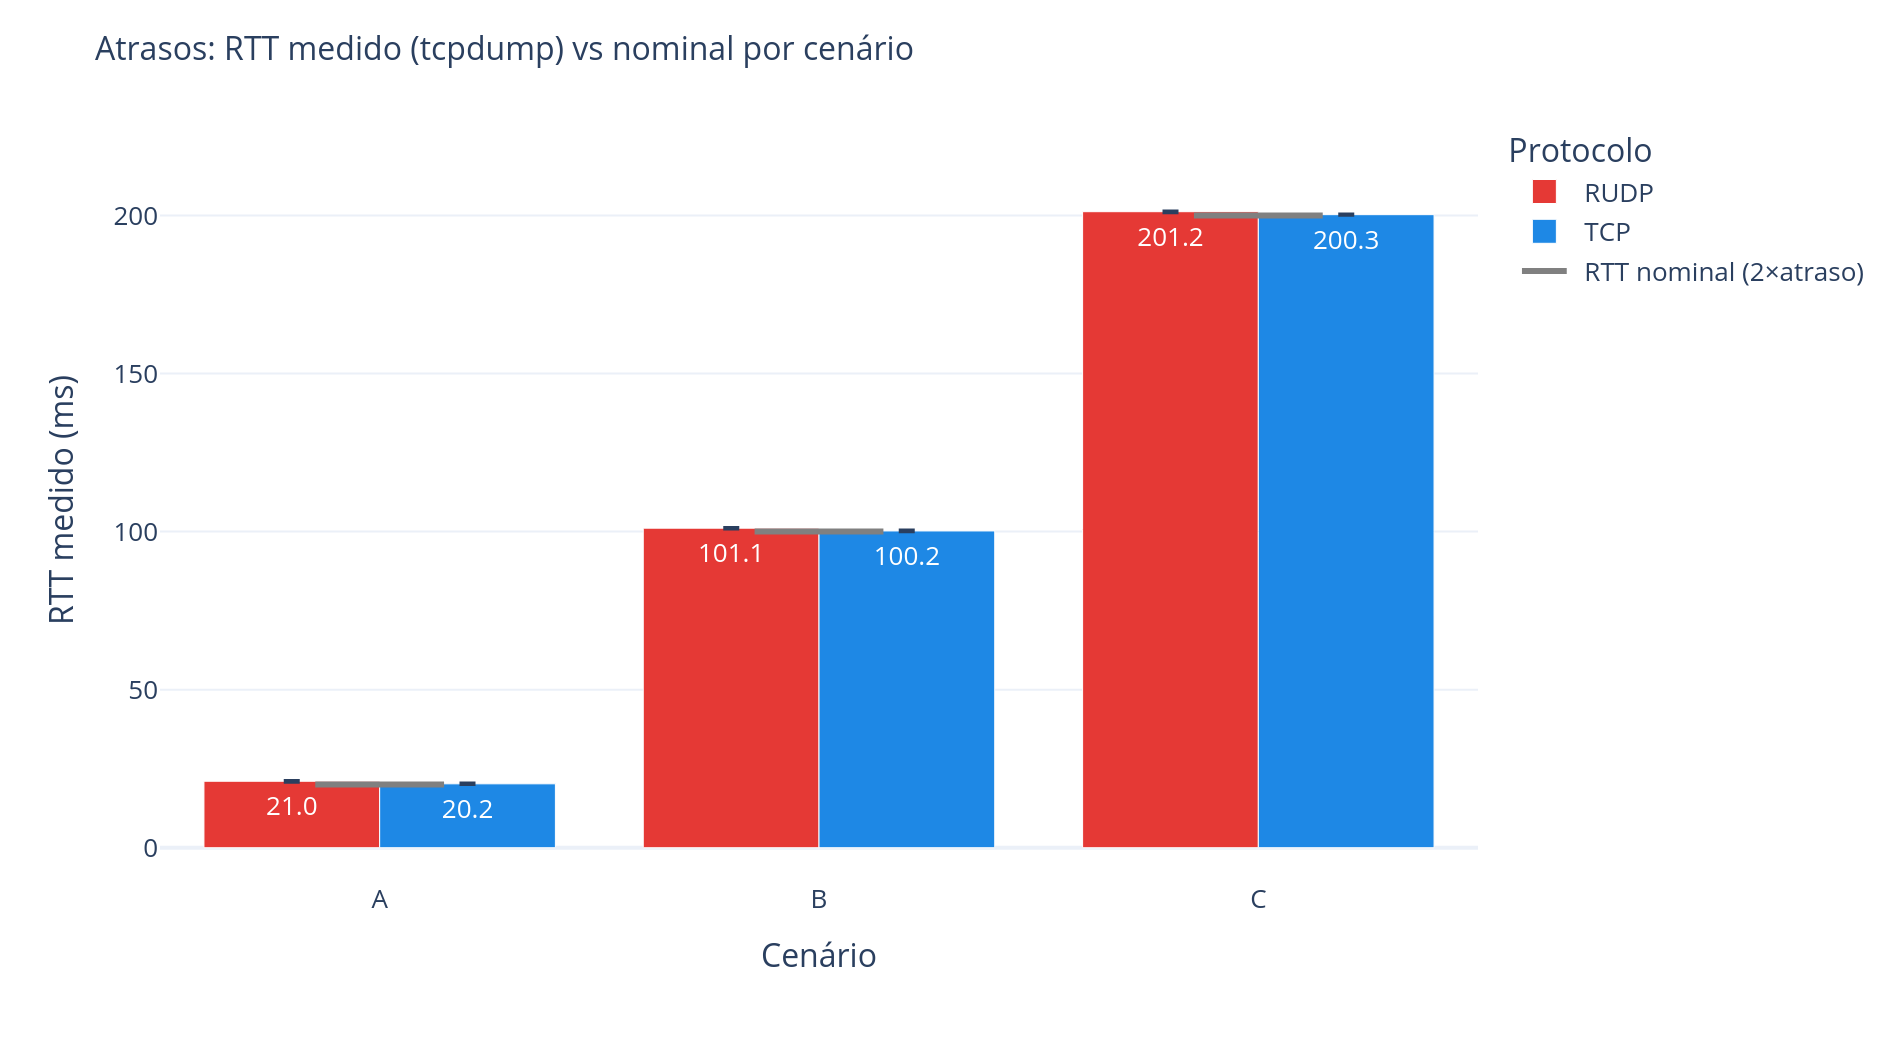
\includegraphics[width=0.85\textwidth]{imgs/fig7_rtt.png}
\caption{Validação do ambiente: RTT empírico (\texttt{tcpdump}) \emph{vs.} RTT nominal esperado.
As medições alinham-se perfeitamente aos parâmetros do \texttt{tc netem}.}
\label{fig:rtt}
\end{figure}

A precisão do simulador de falhas foi aferida diretamente da rede (Figura~\ref{fig:rtt}). 
A partir da captura passiva no servidor, o \emph{Round-Trip Time} foi isolado mensurando o delta 
entre o primeiro segmento (SYN) e a resposta inicial do cliente ao SYN-ACK. Os valores 
medianos empíricos ($\approx$~20, 100 e 200~ms) ratificam a regra $RTT = 2 \times atraso_{one-way}$, 
validando de forma definitiva a calibração do emulador.

\subsection{Perdas de Pacotes: O Efeito da Fragmentação}

\begin{figure}[ht]
\centering
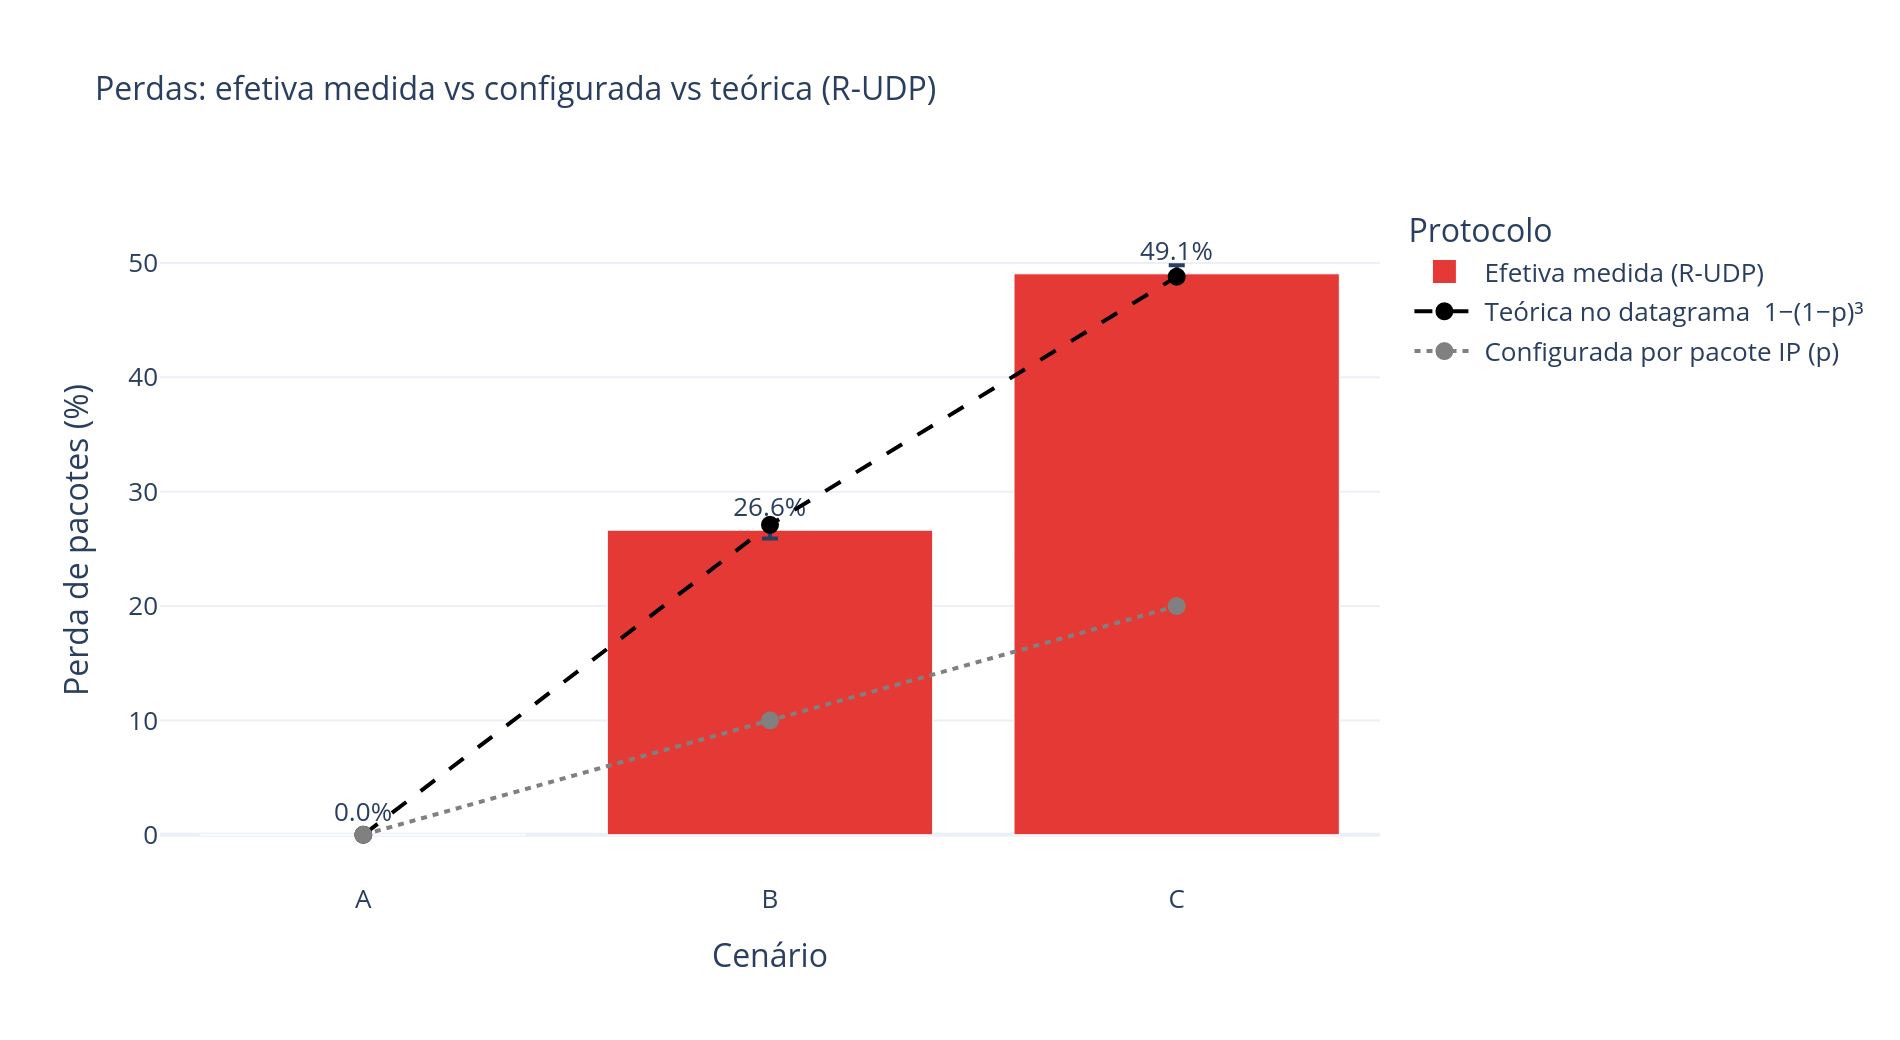
\includegraphics[width=0.85\textwidth]{imgs/fig8_perdas.png}
\caption{Perda de pacotes: efetiva medida pelo R-UDP \emph{vs.} taxa bruta configurada \emph{vs.} 
projeção analítica do modelo $1-(1-p)^3$.}
\label{fig:perdas}
\end{figure}

Como modelado na Seção 3.5, a perda configurada no \texttt{tc} incide de forma restrita sobre os 
pacotes IP, mas o R-UDP sente essa perda no nível do datagrama (após a remontagem dos fragmentos). 
Na Figura~\ref{fig:perdas}, validamos empiricamente este fenômeno matemático. 

O índice de descarte mensurado de forma robusta pela aplicação ($p_{\text{efetiva}} = 1 - 
(\text{ACKs recebidos}) / (\text{Datagramas enviados})$) atinge as marcas de $\approx$~27\% 
e $\approx$~49\% para os cenários B e C, respectivamente. Este registro acompanha com precisão 
cirúrgica a projeção teórica da Equação~\ref{eq:frag} (27,1\% e 48,8\%), distanciando-se amplamente 
da taxa bruta configurada (10\% e 20\%). Conclui-se que o emulador atuou com exatidão, e que a 
arquitetura do \emph{payload} em descompasso com a MTU \textbf{amplifica drasticamente o erro 
aparente}, justificando o severo estresse imposto à malha de confiabilidade do R-UDP.

\subsection{Retransmissões e Overhead de Banda}

\begin{figure}[ht]
\centering
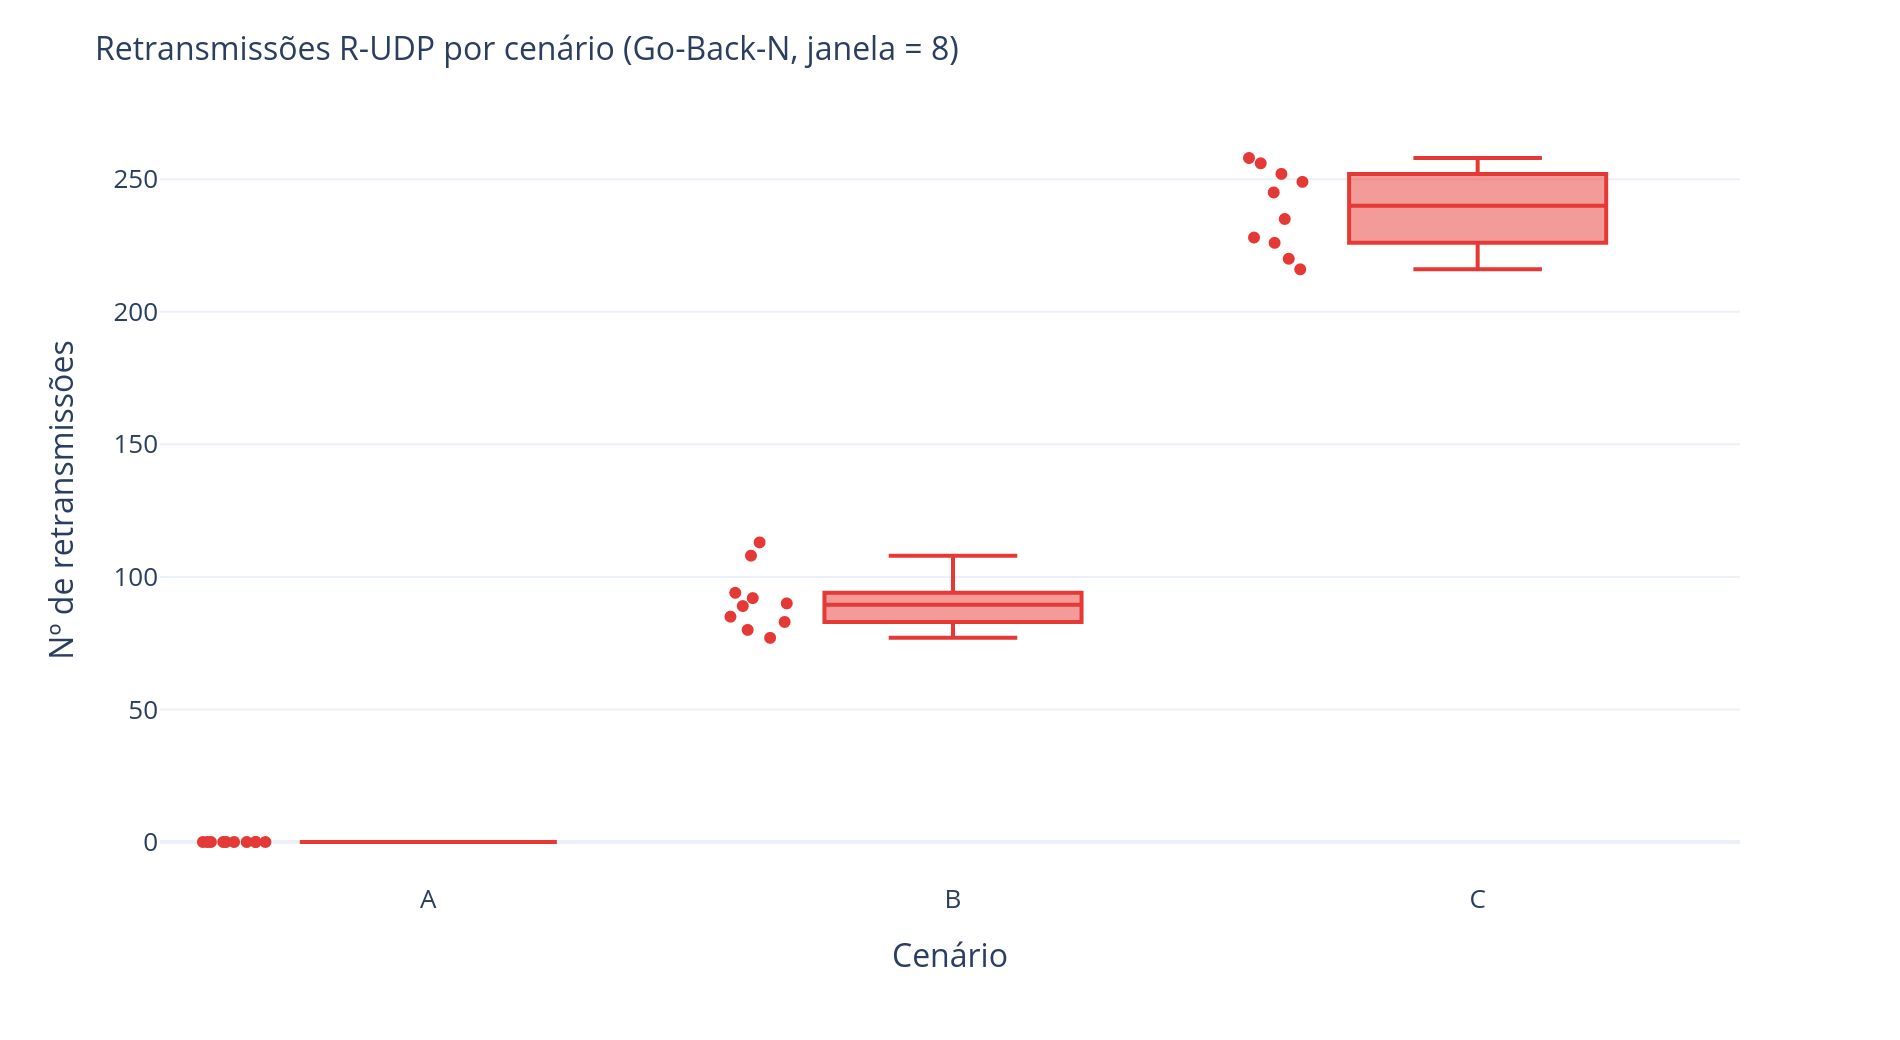
\includegraphics[width=0.85\textwidth]{imgs/fig3_retransmissoes.png}
\caption{Ativação da lógica de confiabilidade R-UDP: disparos de \emph{timeouts} acionando o 
recuo da janela Go-Back-N.}
\label{fig:retx}
\end{figure}

\begin{figure}[ht]
\centering
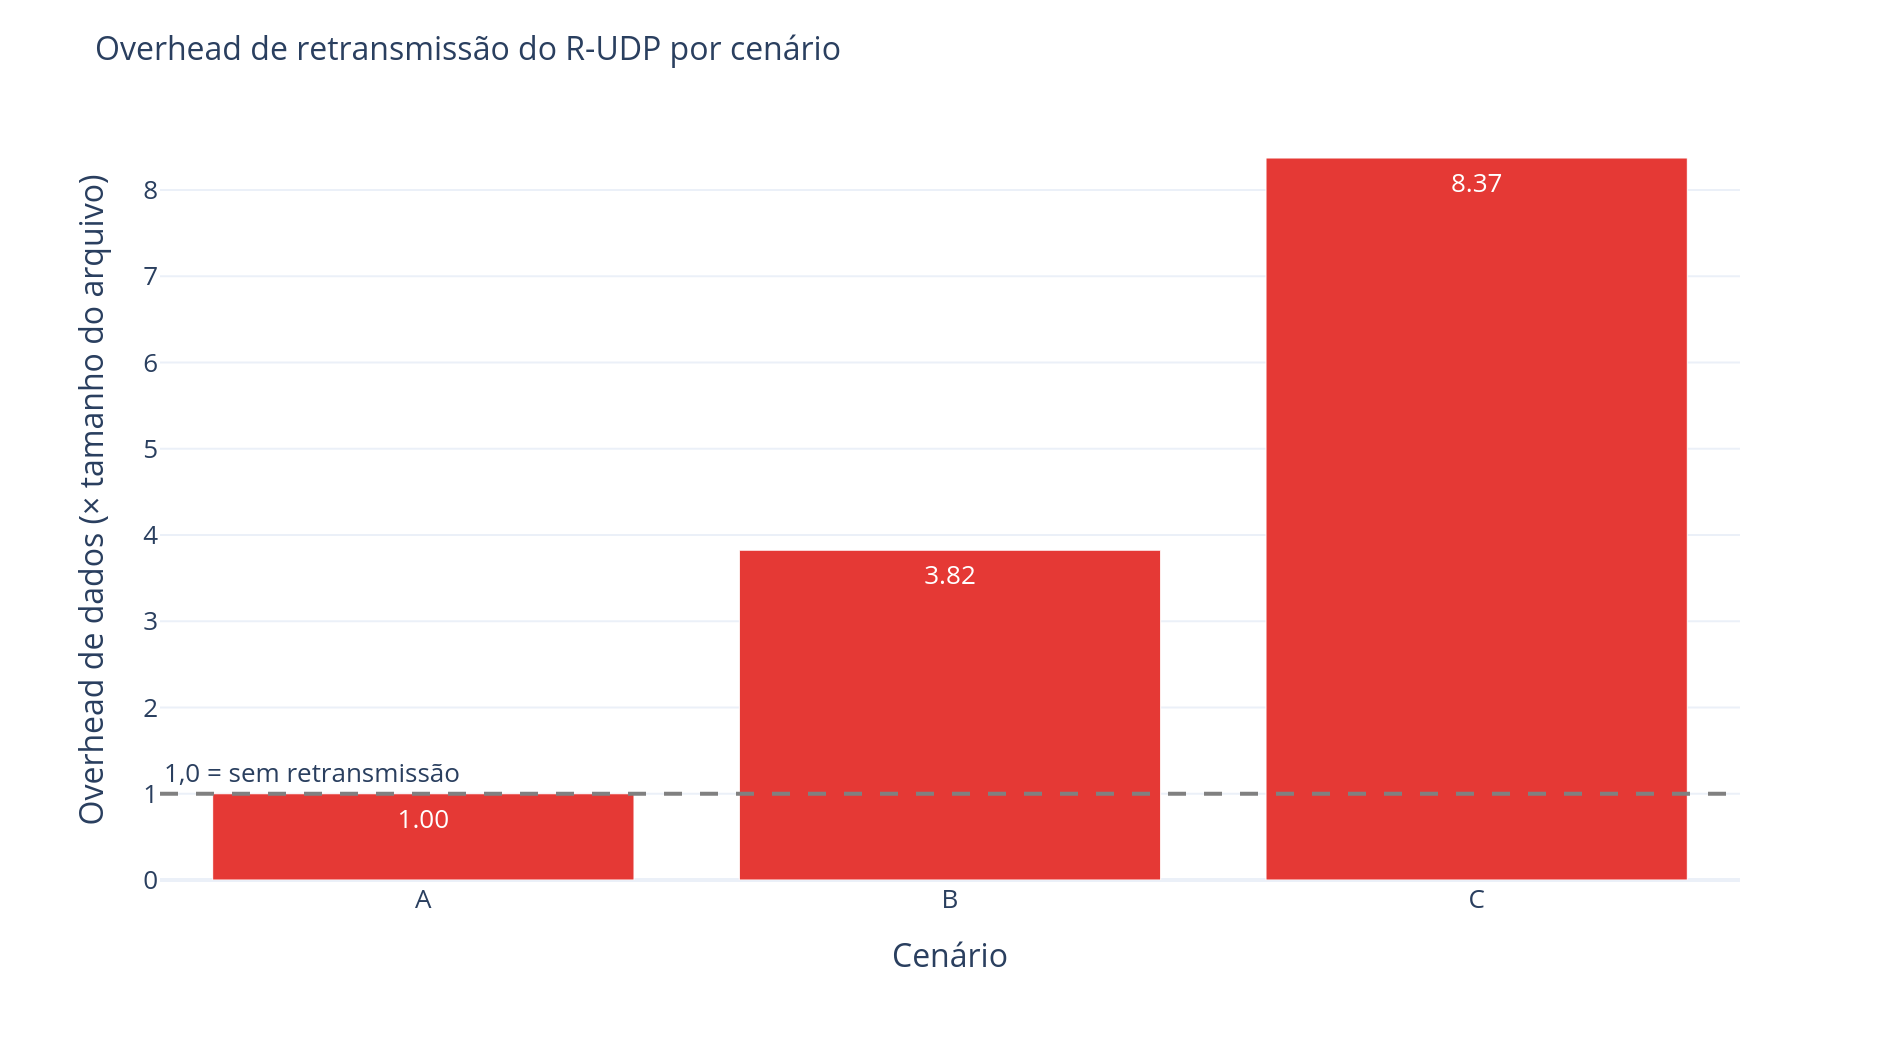
\includegraphics[width=0.85\textwidth]{imgs/fig4_overhead.png}
\caption{\emph{Overhead} bruto de tráfego do R-UDP, evidenciando o custo da redundância 
inerente à estratégia Go-Back-N.}
\label{fig:overhead}
\end{figure}

O sacrifício exigido pela recuperação em nível de aplicação é dissecado nas 
Figuras~\ref{fig:retx} e~\ref{fig:overhead}. Os eventos de retransmissão escalam de zero 
(Cenário A) para medianas de 90 (B) e 240 (C). Impulsionado pela amplificação da MTU discutida 
anteriormente, o \emph{overhead} volumétrico --- a razão entre blocos transmitidos e blocos 
úteis --- escala de $1,0\times$ (eficiência máxima em A) para exorbitantes $3,8\times$ (B) e 
$8,4\times$ (C). Este fardo é o traço intrínseco do Go-Back-N, apontando para a urgência da 
substituição futura para uma estratégia baseada em \emph{Selective Repeat}.

Importante frisar que o TCP exibe estatisticamente, no nível de aplicação (Sockets), um 
\emph{overhead} utópico de $1,0\times$. Isso ocorre exclusivamente por sua natureza opaca; 
as retransmissões são tratadas isoladamente pelo núcleo do sistema, desafiando a observabilidade 
do protocolo e motivando a técnica de integração de dados abordada a seguir.

\subsection{Integração de Dados: Comparação entre a Aplicação e o TCPDump}

Atendendo estritamente ao critério de integração de dados do projeto, esta seção realiza a 
\textbf{validação cruzada} entre os eventos mapeados pela instrumentação \emph{user-space} (JSONL) e a 
telemetria absoluta dos enlaces provida pelo analisador de pacotes (\texttt{tcpdump}).

\begin{figure}[ht]
\centering
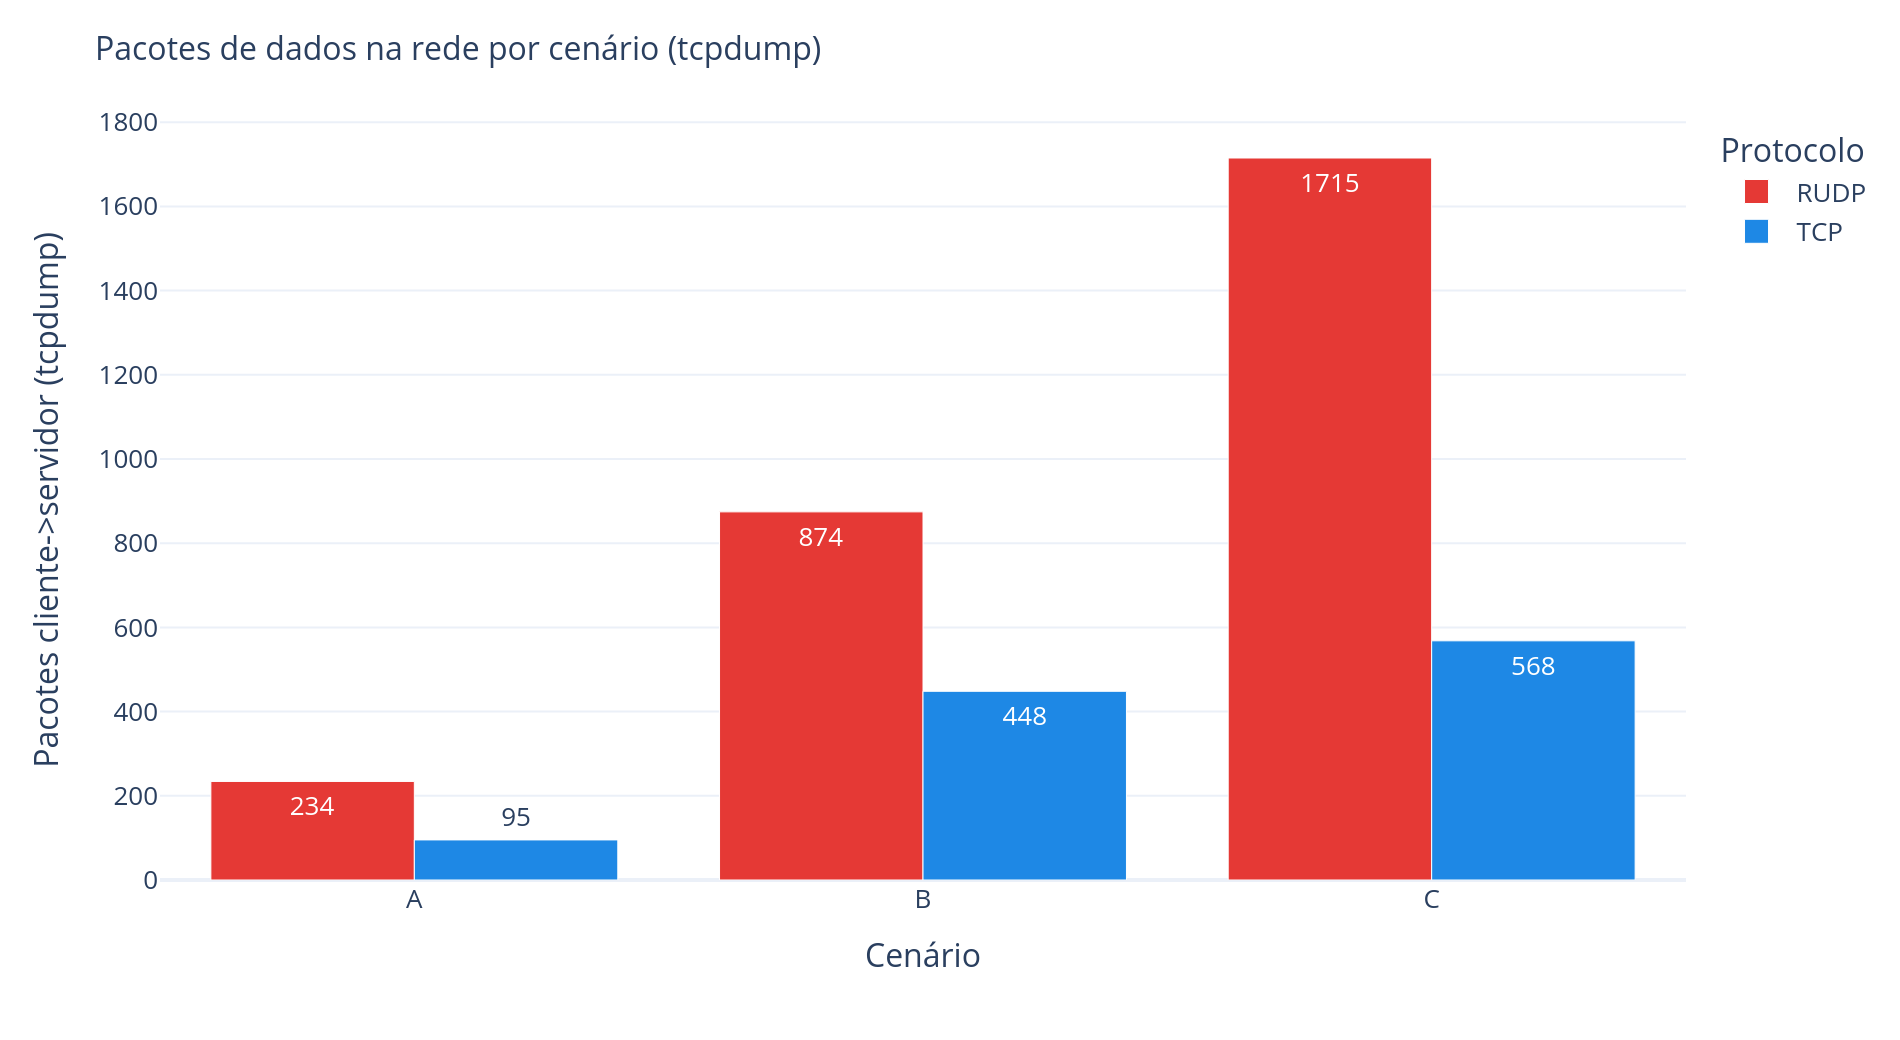
\includegraphics[width=0.85\textwidth]{imgs/fig5_pacotes_rede.png}
\caption{O comportamento oculto do TCP exposto: contagem bruta de tráfego 
cliente$\rightarrow$servidor registrada pelo \texttt{tcpdump}.}
\label{fig:pacotes}
\end{figure}

A Figura~\ref{fig:pacotes} funciona como a contraprova externa do estudo. Ao auditar diretamente a rede, 
desmascaramos o aparente fluxo imaculado do TCP. Observa-se que a contagem total de pacotes TCP escalona 
agressivamente sob perda (Cenário C), comprovando empiricamente que a confiabilidade impõe retransmissões 
massivas também no \emph{kernel}, independentemente do que o \emph{Socket} decide reportar ao \emph{software}.

\begin{figure}[ht]
\centering
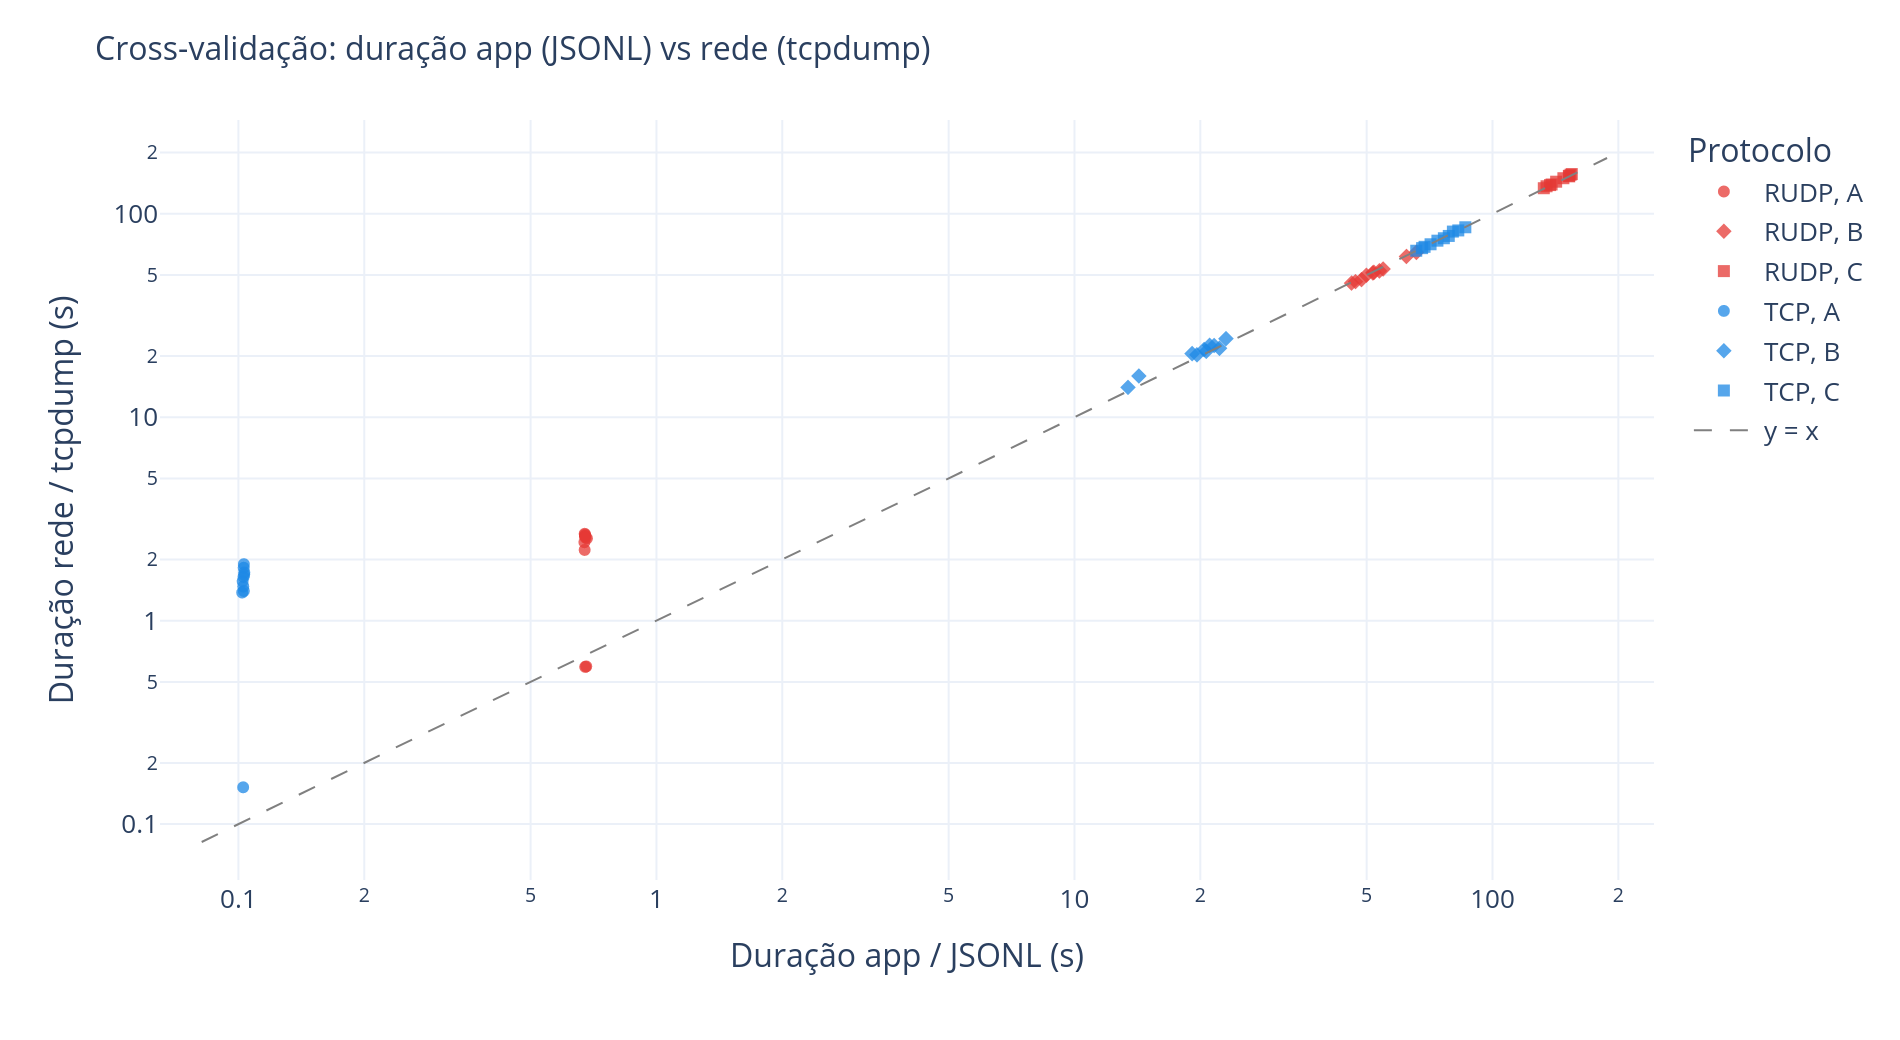
\includegraphics[width=0.85\textwidth]{imgs/fig6_crossval.png}
\caption{Dispersão para validação cruzada do tempo de transferência (Aplicação \emph{vs.} \texttt{tcpdump}). 
A convergência para a bissetriz $y = x$ chancela a precisão dos registros internos.}
\label{fig:crossval}
\end{figure}

Finalmente, a Figura~\ref{fig:crossval} correlaciona a duração total registrada pelos relógios da 
aplicação contra os marcadores temporais da captura de pacotes. Nos cenários penalizados (B e C), os 
pontos ancoram-se sobre a linha de identidade ($y = x$), ostentando uma divergência técnica inferior a 5\%. 
O deslocamento sutil observado no Cenário A é oriundo unicamente do \emph{overhead} estático de encerramento 
de sessões (cerca de 1,4~s), o qual domina percentualmente apenas quando a transferência útil é sub-segundo. 
Logo, os relatórios gerados pela aplicação R-UDP são certificados como estatisticamente íntegros.

\subsection{Prova do campo \texttt{X-Custom-Auth} na captura}

Conforme demandado pelas diretrizes do projeto, o cabeçalho \texttt{X-Custom-Auth} composto 
por ``matrícula + nome'' deve trafegar explicitamente sobre a rede, sendo rastreável através 
de inspeção profunda de pacotes. Abaixo, reproduz-se o \emph{hexdump} de uma captura real 
(\texttt{tcpdump -X}), demonstrando a presença legível da \emph{magic string} \texttt{RDFT} 
e as credenciais, garantindo a conformidade total com o requisito de autenticação de carga útil.

\begin{verbatim}
0x0030:  2977 f920 5244 4654 0000 0000 0010 0000  )w..RDFT........
0x0050:  0000 3230 3236 3130 3131 3431 3020 414e  ..20261011410.AN
0x0060:  5448 4f4e 5920 4952 4c41 4e20 4d41 5251  THONY.IRLAN.MARQ
0x0070:  5545 5320 4c55 5a00 0000 0000 0000 0000  UES.LUZ.........
\end{verbatim}

Evidências suplementares (telas do Wireshark via filtro \texttt{frame contains "ANTHONY"}) e os 
respectivos arquivos \texttt{.pcap} foram anexados ao repositório institucional do projeto em 
\texttt{results/evidence/}.

\section{Síntese e Respostas aos Requisitos}

\textbf{O que a aplicação mediu condiz com o \texttt{tcpdump}?} Plenamente. Através da técnica de integração 
de dados provamos que a cronometragem converge (Figura~\ref{fig:crossval}) e que as instâncias de retransmissão 
escalam em ambas as topologias conforme previsto matematicamente (Figura~\ref{fig:pacotes}). O R-UDP, ao contrário 
do TCP, possui o mérito de expor essa carga analítica diretamente para a aplicação.

\textbf{Qual o custo da confiabilidade em espaço de usuário?} O custo mostrou-se condicionado à qualidade do canal. 
Em regime ótimo, a penalidade é negligenciável (fração de segundo). Em zonas de intenso descarte, o 
custo transparece severamente em tempo (degradação de $1,9\times$ frente ao TCP no Cenário C) e em redundância 
de tráfego ($8,4\times$ mais envios). O TCP aparenta melhor resiliência em tempo pois converte a perda em 
estrangulamento direto de vazão, minimizando as rodadas cegas de tráfego injetado na rede.

\textbf{O algoritmo Go-Back-N é adequado sob perda alta?} A rigor, sua eficácia é questionável. Ele preserva o postulado da 
integridade (100\% de sucesso demonstrado), mas aniquila o \emph{goodput} da rede ao forçar a retransmissão 
bruta de segmentos validados. Conjugado à modelagem de amplificação do erro causada pela MTU, 
o Go-Back-N provou-se altamente inadequado para enlaces agressivos, abrindo precedentes inequívocos para 
a adoção mandatória de lógicas de \emph{Selective Repeat}.

\section{Conclusão e Trabalhos Futuros}

Este trabalho materializou o dimensionamento empírico da confiabilidade de redes. Projetamos e instrumentamos 
arquiteturas de transporte em contêineres e validamos, com cruzamento de \emph{logs} e topologias de interceptação 
(\texttt{tcpdump}), a exata assimetria comportamental entre o tratamento nativo e abstraído de erros (TCP) 
e a mecânica exposta em camada de aplicação (R-UDP / Go-Back-N). Isolamos e provamos matematicamente que o 
limite físico do enlace (MTU) atua como um severo catalisador de falhas para datagramas expandidos.

Para a próxima fase deste ciclo de pesquisa (Modelagem Estocástica), o arcabouço lógico do R-UDP aqui ratificado 
será traduzido para um simulador de eventos discretos fundamentado em \texttt{SimPy}. O modelo empírico 
sedimentado por este relatório proverá os parâmetros de base (\emph{baselines}) que permitirão validar 
estatisticamente as projeções puramente teóricas simuladas em ambiente computacional no futuro.

\bibliographystyle{sbc}
\bibliography{references}

\end{document}